\subsection{Intuition and Assumptions}
\label{intuitionSection}
    Since data bus is $16-bits$ in width i.e. $word$, so the following sizes are in terms of $words$.
    
    Since we are dealing with ONE main memory that contains all the Data and Instructions,
    and two caches one for Data and the other is for Instructions.

    This Design proposes to divide the Main memory into two parts, one for Data and one for Instructions,
    the upper most part is saved for Data from \textit{address} $00000000000$ to $01111111111$, while the Instructions
    \textit{address} starts from $10000000000$ to $11111111111$.

    Considering this, the $LSB$ of the address will indicate whether that address is corresponding to an instruction ($1$) or data ($0$).

    These assumptions allow us to:
    \begin{itemize}
        \item Limit collisions (conflicts) since for each Cache the tag size is reduced
            to only two bits since the actual address is 10 bits.
        \item Create an internal pipeline between the instruction cache and data cache,
            since the instruction cache is used only for reading, and filled periodically, more on 
            that on section \nameref{workflowSection}.
        \item No dirty bit array is used for instruction cache.
    \end{itemize}
     
\subsection{Caches Size}
    What is Given:
    \begin{itemize}
        \item Main memory: $4KB = 2^{12}B =2^{11} W$
        \item Cache Size: $512 Bytes = 256Words$
        \item Block Size: $16B = 8W$
        \item Number of Rows/Slots: $32$
        \item Number of Caches: $2$ one for Data and one for Instructions.
    \end{itemize}

    Sizes:
    \begin{itemize}
        \item Each Cache is $256Words$
        \item Tags are 2 bits in width.
        \item Validity is only 1 bit.
        \item Dirty bit is used only in case of Data cache.
        \item Extra bits required in total: $32*(2+1) + 16*(1) = 112bits$
    \end{itemize}


\subsection{Workflow}
\label{workflowSection}
    \subsubsection{General Cache Design}
    As proposed in the \nameref{intuitionSection} section, two caches exist in the design.

    In order to increase efficiency; we propose this fig.\ref{fig:cacheDesign}:
    \begin{itemize}
        \item Initially the instruction cache is filled with the first $Block$.
        \item The program will start working as usually\dots
        \item If No memory instruction is produced, this means the Memory is Ideal..
        \item The Cache Controller requests more $Blocks$ of Instructions from main memory.
        \item Meanwhile if Data is required from memory to be read or written, it will wait 
            until the current block is retrieved then the required $Data$ will be provided.
        \item Then the $Data$ request will be full-filled.
        \item This means that Data Memory has higher priority unless the instruction cache is empty.
    \end{itemize}

    The following algorithm may make things more clear\dots

    \begin{algorithm}
        \SetAlgoLined
        \While{True}{
            \uIf{Instruction Cache is Empty}{
                Fetch the Next Instruction.\;
            }
            \uElseIf{Memory is Free to be Used}{
                Fetch the Next Instruction.\;
            }
            \Else{
                \uIf{there is a Data Memory Instruction}{
                    \uIf{Memory is Busy}{
                        Queue it next\;
                    }\Else{
                        Operate Now\;
                    }
                }
            }
        }
        \caption{Cache Controller}
        \end{algorithm}
    
    \vspace{1cm}
    What makes this algorithm efficient is these two information, One: the Instruction cache
    can be written periodically, Two: the Rate of Memory Instruction is very low and the Number
    of memory instruction (such as $SW$ and $LD$) is less than other Instructions.
    
    \subsubsection{Data Cache Design}

    In the following flowchart fig.\ref{fig:dataCache} we illustrate how read and write operations are
    handled in our system.\newline

    Notes:
    \begin{itemize}
        \item These operations are related to $Data$ cache.
        \item When Valid bit equals 0, this means it's not valid, and vv.
        \item When Dirty bit equals 0. this means the block is not modified, and vv.
        \item $Circle A$ is responsible for reading from main memory.
        \item $Circle B$ is responsible for writing into main memory (Replacement).
        \item Replacement occurs only when read is demanded let's see why:
            \begin{itemize}
                \item when dirty bit is set, and that exact same block is needed for read or write operation
                \item If it's needed for read operation then the old block will be written first,
                    then the ordered block will be read, this is ordinary Replacement.
                \item and if it's needed for write operation, then if it's not valid or missed ordinary Replacement
                is requested,
                \item but if it was valid and tag is matched then we don't need to check the dirty bit
                \textbf{data can be overwritten without updating the main memory} and the dirty bit is set anyway.
            \end{itemize}
    \end{itemize}
    
    \begin{figure}
        \centering
        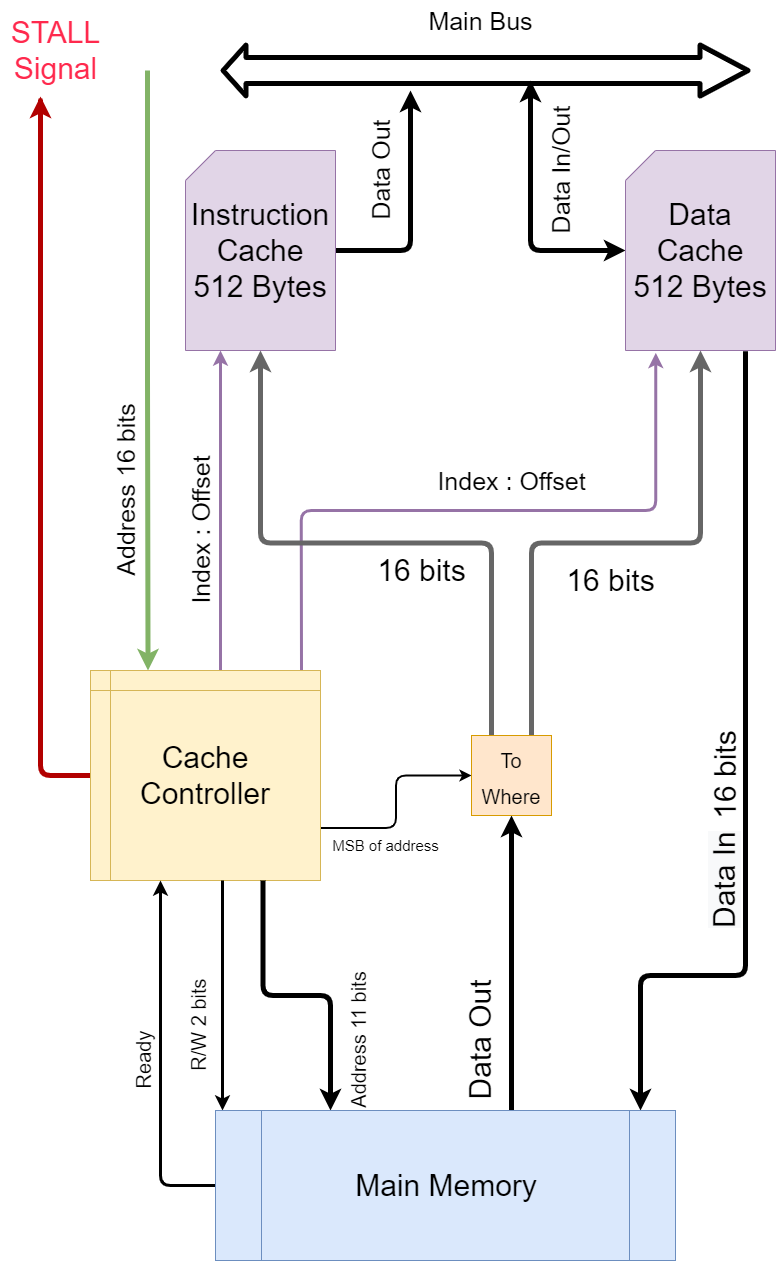
\includegraphics[width=0.5\textwidth]{images/cache/full_cache_design.png}
        \caption{Cache Design}
        \label{fig:cacheDesign}
    \end{figure}


    \begin{figure}
        \centering
        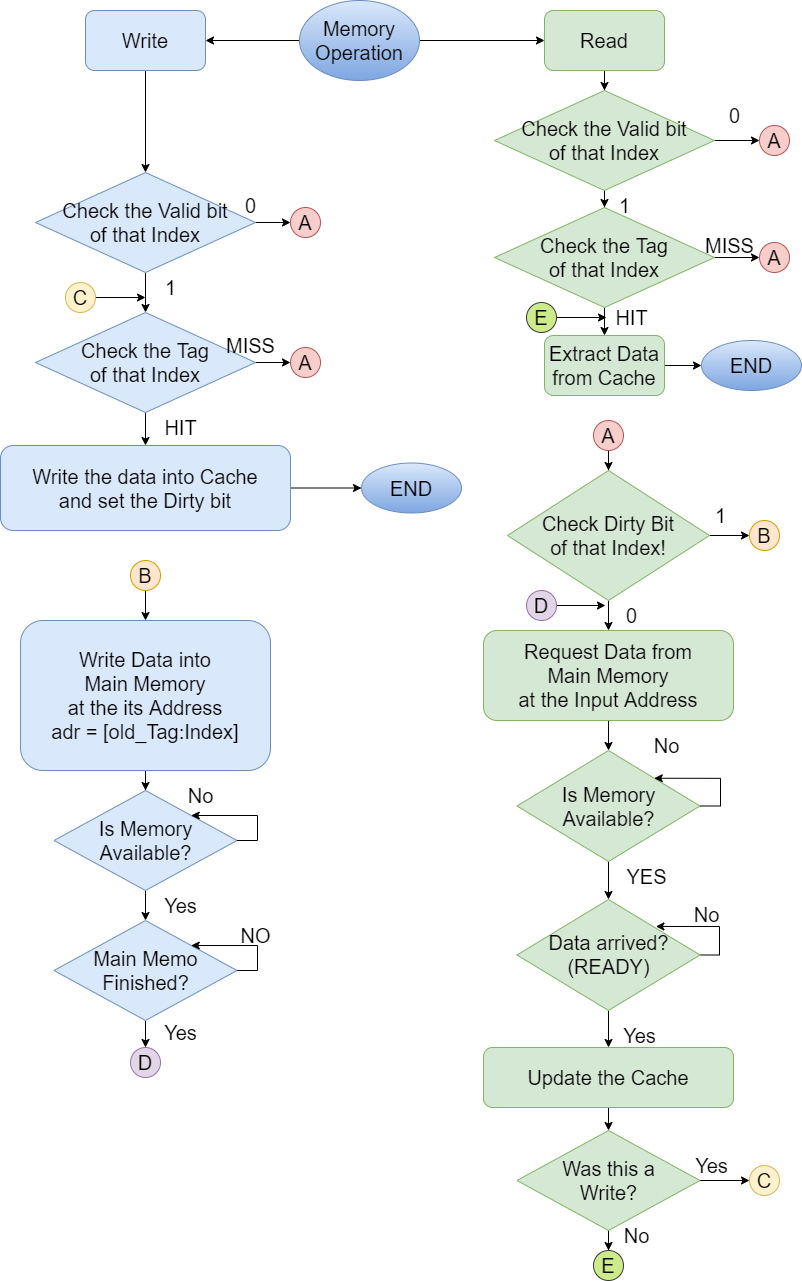
\includegraphics[width=0.8\textwidth]{images/cache/cache_system_flowchart.png}
        \caption{Data Cache R/W}
        \label{fig:dataCache}
    \end{figure}

